\subsection{B6U: Ungesteuerter Dreiphasen-Brückengleichrichter}

% --- bestehende Grafik: Schaltung ---
\begin{center}
    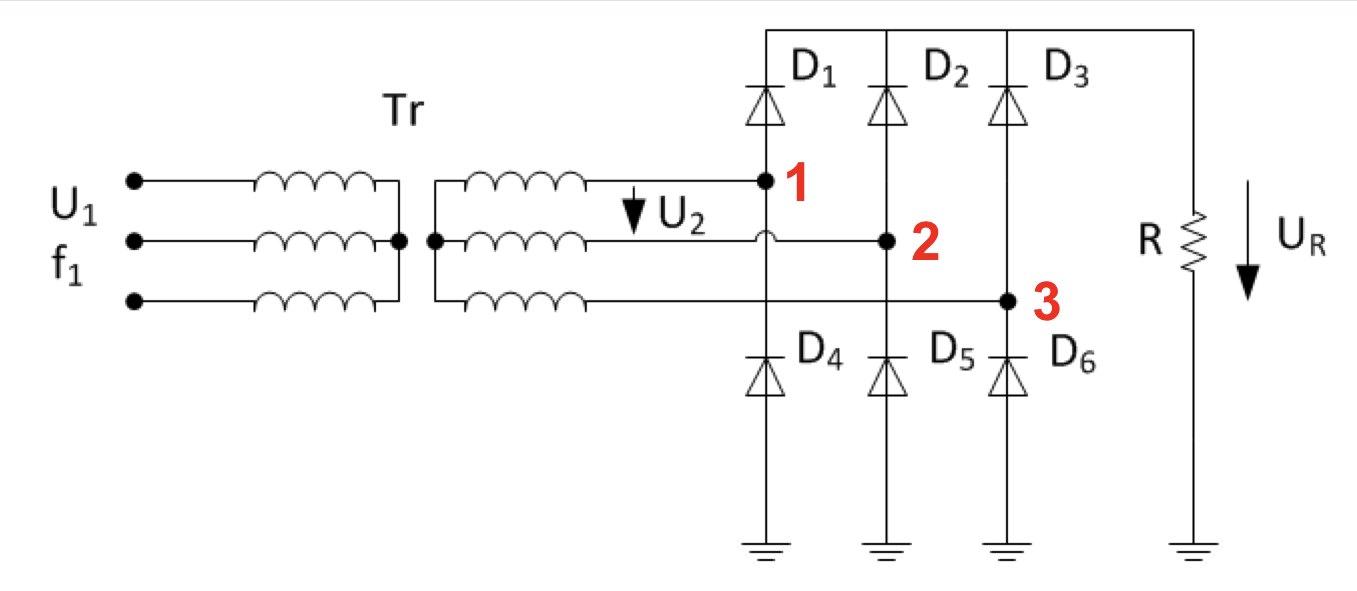
\includegraphics[width=0.65\linewidth]{images/B6U.png}
\end{center}

Der ungesteuerte Dreiphasen-Brückengleichrichter besteht aus sechs Dioden
und nutzt jeweils die beiden momentanen Leiterspannungen mit größtem Betrag.
Die Pulszahl beträgt $p=6$.

Eingangsspannungen:
\[
u_{ab}(t),\; u_{bc}(t),\; u_{ca}(t)
\]
mit:
\begin{itemize}
\item $U_{LL}$: Effektivwert der Leiterspannung,
\item $\hat U_{LL} = \sqrt{2} U_{LL}$: Scheitelwert der Leiterspannung,
\item $\omega = 2\pi f$: Kreisfrequenz,
\item $f$: Netzfrequenz.
\end{itemize}

Momentane Ausgangsspannung:
\[
u_d(t) = \max \{ u_{ab}(t),\, u_{bc}(t),\, u_{ca}(t),\, 0 \}
\]

Mittelwert der Gleichspannung:
\[
\cbl{\overline{u_d}
= \frac{3\sqrt{2}}{\pi} U_{LL}}
\]

Effektivwert der Gleichspannung (ideal, ohne Überlappung):
\[
\cbl{U_{d,\mathrm{RMS}}
= \sqrt{\frac{1}{2\pi}\int_0^{2\pi} u_d^2(\gamma)\, d\gamma}}
\]

Mittelwert des Gleichstroms bei ohmscher Last $R$:
\[
\cbl{I_d = \frac{\overline{u_d}}{R}
= \frac{3\sqrt{2}}{\pi}\frac{U_{LL}}{R}}
\]

Effektivwert des Gleichstroms:
\[
\cbl{I_{d,\mathrm{RMS}} = \frac{U_{d,\mathrm{RMS}}}{R}}
\]

Leistungsaufnahme an ohmscher Last:
\[
\cbl{P = R I_{d,\mathrm{RMS}}^2}
\]

Ripple-Frequenz der Gleichspannung:
\[
\cbl{f_r = p f = 6 f}
\]

Ripple-Faktor:
\[
\cbl{r = \frac{\sqrt{U_{d,\mathrm{RMS}}^2 - \overline{u_d}^2}}{\overline{u_d}}}
\]

Eigenschaften:
\begin{itemize}
\item Sehr geringe Restwelligkeit der Gleichspannung.
\item Hohe Gleichspannungsqualität.
\item Sehr gute Ausnutzung der Netzspannung.
\item Standard-Gleichrichter in Industrieanwendungen.
\end{itemize}

% --- bestehende Grafik: Spannungsverlauf ---
\begin{center}
    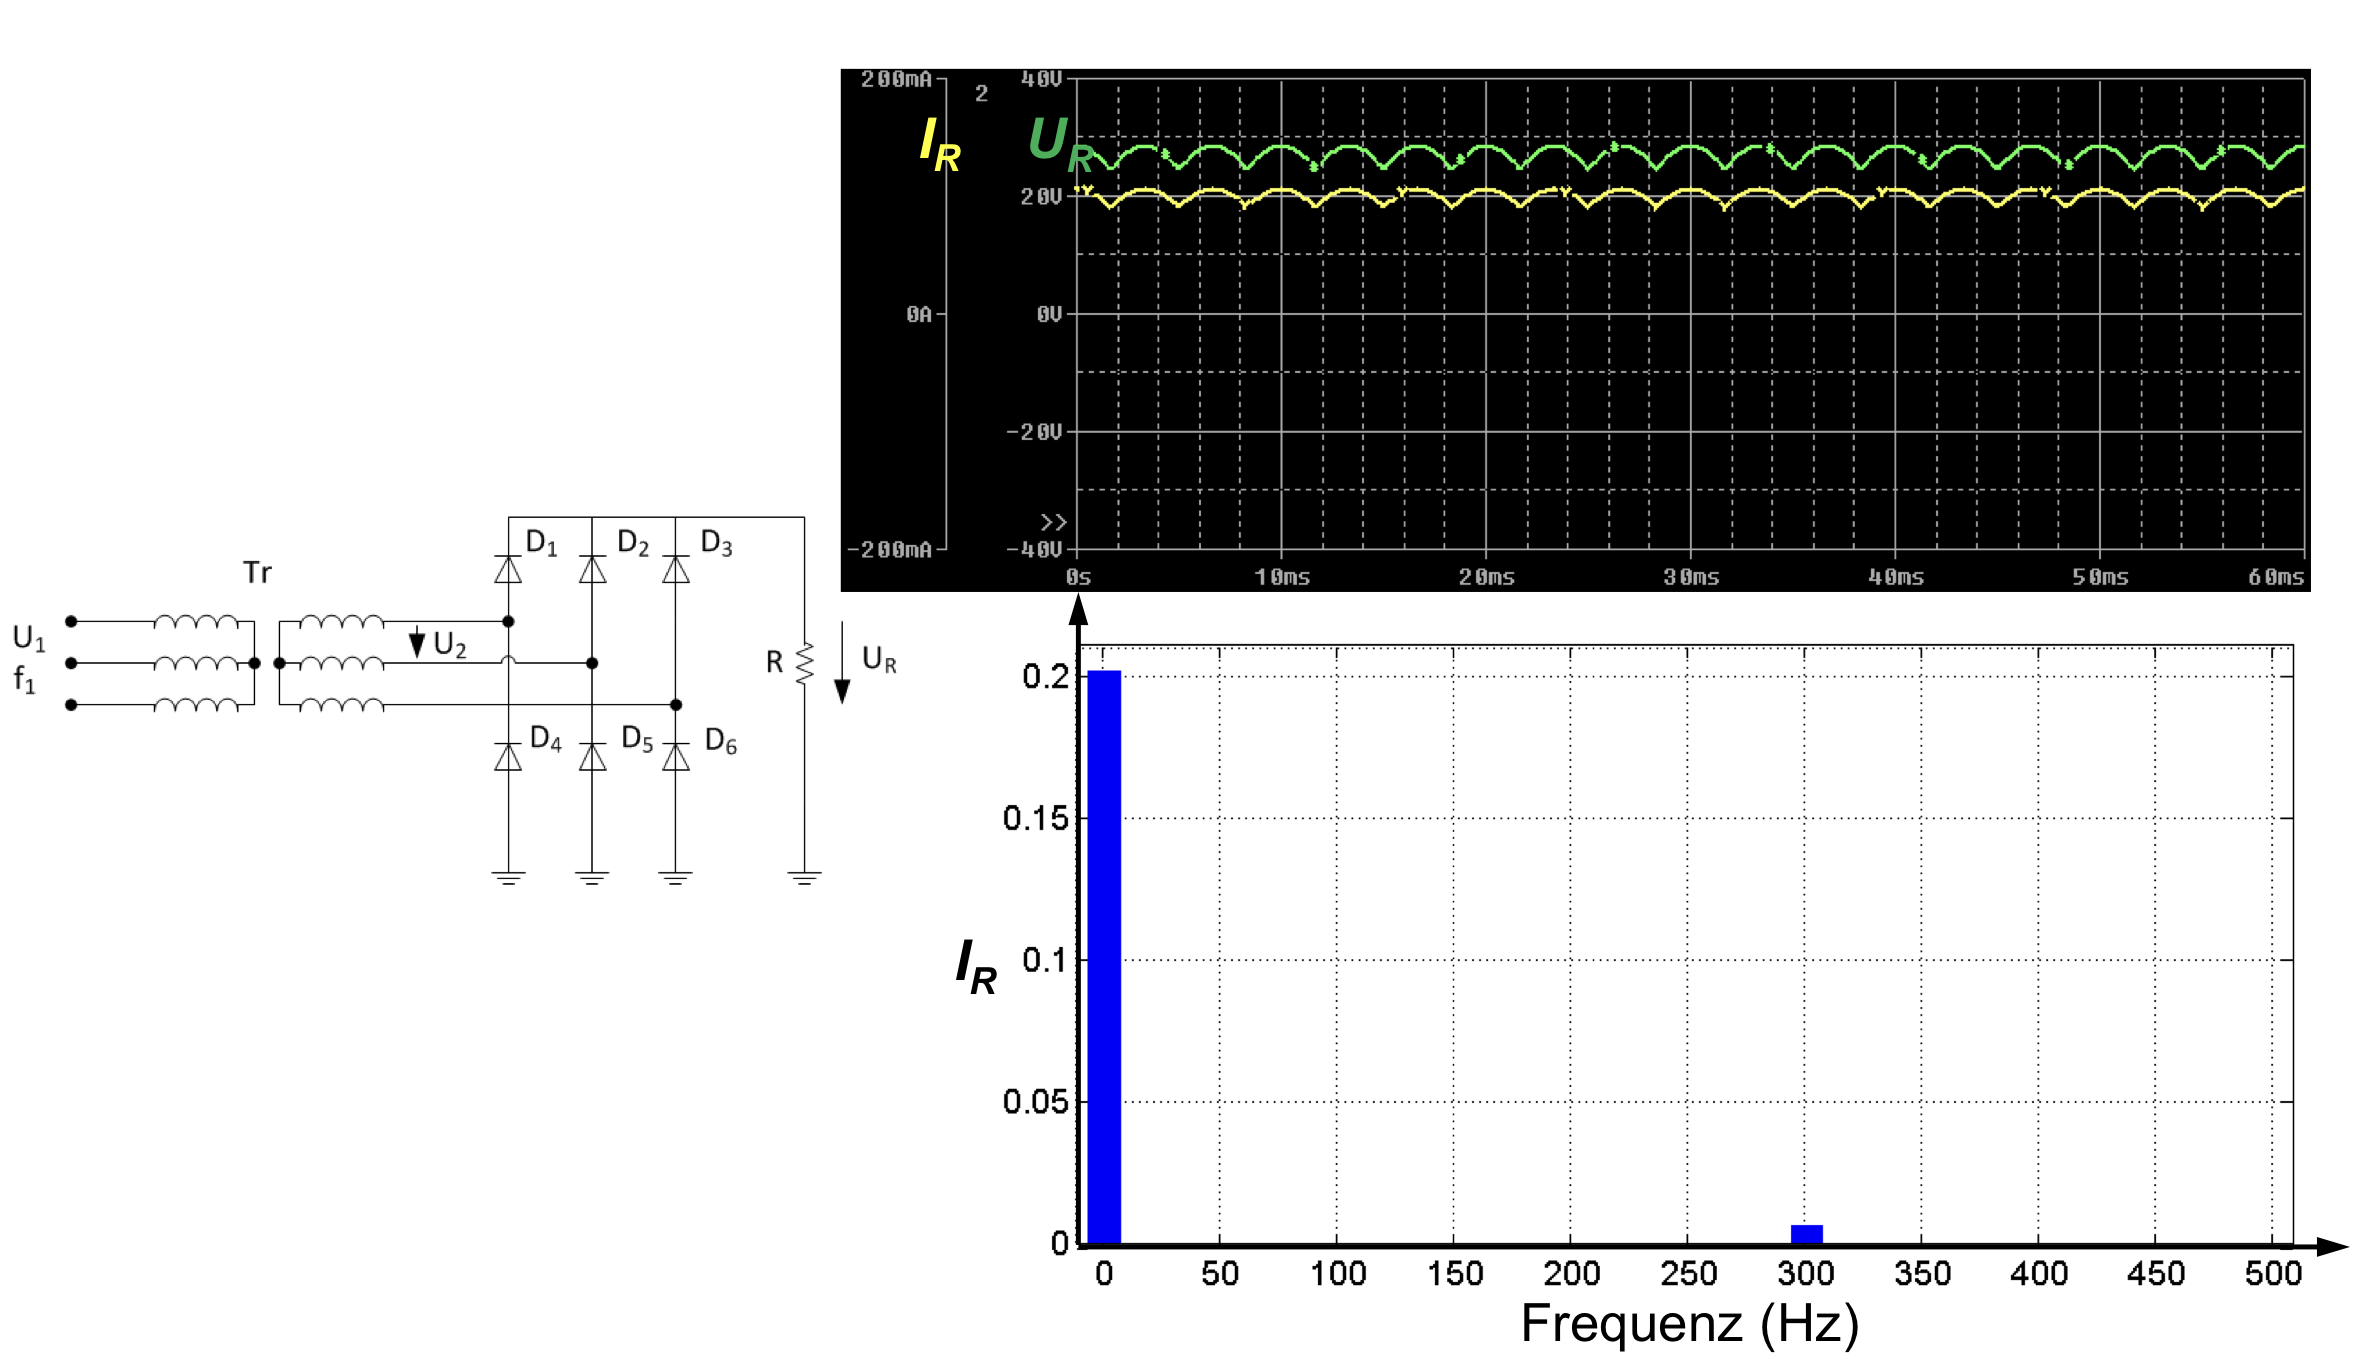
\includegraphics[width=0.85\linewidth]{images/B6U_verlauf.png}
\end{center}

\subsection{B6C: Gesteuerter Dreiphasen-Brückengleichrichter}

% --- bestehende Grafik: Schaltung ---
\begin{center}
    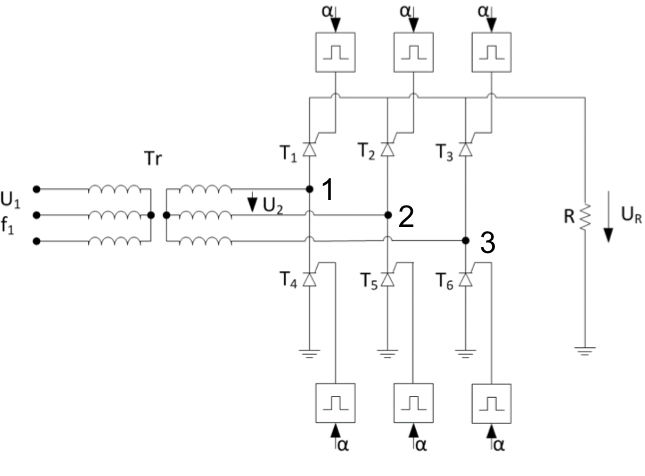
\includegraphics[width=0.65\linewidth]{images/B6C.png}
\end{center}

Der gesteuerte Dreiphasen-Brückengleichrichter ersetzt die Dioden durch Thyristoren.
Der Leitbeginn jedes Ventils wird über den Zündwinkel $\alpha$ gesteuert.

Eingangsspannungen:
\[
u_{ab}(t),\; u_{bc}(t),\; u_{ca}(t)
\]
mit:
\begin{itemize}
\item $U_{LL}$: Effektivwert der Leiterspannung,
\item $\hat U_{LL} = \sqrt{2} U_{LL}$: Scheitelwert der Leiterspannung,
\item $\omega = 2\pi f$: Kreisfrequenz,
\item $f$: Netzfrequenz.
\end{itemize}

Leitbedingung:
\[
\boxed{\omega t \ge \alpha}
\]

Momentane Ausgangsspannung:
\[
u_d(t) = u_{k\ell}(t)
\]
mit:
\begin{itemize}
\item $u_{k\ell}(t)$: jeweils aktive Leiterspannung des gerade leitenden Ventilpaares.
\end{itemize}

Mittelwert der Gleichspannung (ideal, ohne Überlappung):
\[
\cbl{\overline{u_d}
= \frac{3\sqrt{2}}{\pi} U_{LL} \cos\alpha}
\]

Stellbereich:
\[
0 \le \alpha \le \pi
\]

Grenzfälle:
\[
\alpha = 0 \Rightarrow \overline{u_d} = \frac{3\sqrt{2}}{\pi} U_{LL}
\]
\[
\alpha = \frac{\pi}{2} \Rightarrow \overline{u_d} = 0
\]
\[
\alpha > \frac{\pi}{2} \Rightarrow \overline{u_d} < 0 \quad \text{(Rückspeisebetrieb möglich)}
\]

Mittelwert des Gleichstroms bei ohmscher Last $R$:
\[
\cbl{I_d = \frac{\overline{u_d}}{R}
= \frac{3\sqrt{2}}{\pi}\frac{U_{LL}}{R}\cos\alpha}
\]

Effektivwert der Gleichspannung:
\[
\cbl{U_{d,\mathrm{RMS}}
= \sqrt{\frac{1}{2\pi}\int_0^{2\pi} u_d^2(\gamma)\, d\gamma}}
\]

Leistungsaufnahme an ohmscher Last:
\[
\cbl{P = R I_{d,\mathrm{RMS}}^2}
\]

Leistungsfaktor bei ohmscher Last:
\[
\cbl{\lambda = \frac{P}{\sqrt{3} U_{LL} I_{L,\mathrm{RMS}}}}
\]
mit:
\begin{itemize}
\item $I_{L,\mathrm{RMS}}$: Effektivwert des Leiterstroms.
\end{itemize}

Eigenschaften:
\begin{itemize}
\item Stellbare Gleichspannung über den Zündwinkel $\alpha$.
\item Mittelwert proportional zu $\cos\alpha$.
\item Rückspeisebetrieb für $\alpha > 90^\circ$.
\item Wichtigster gesteuerter Industrie-Gleichrichter.
\end{itemize}

% --- bestehende Grafik: Zeitverlauf ---
\begin{center}
    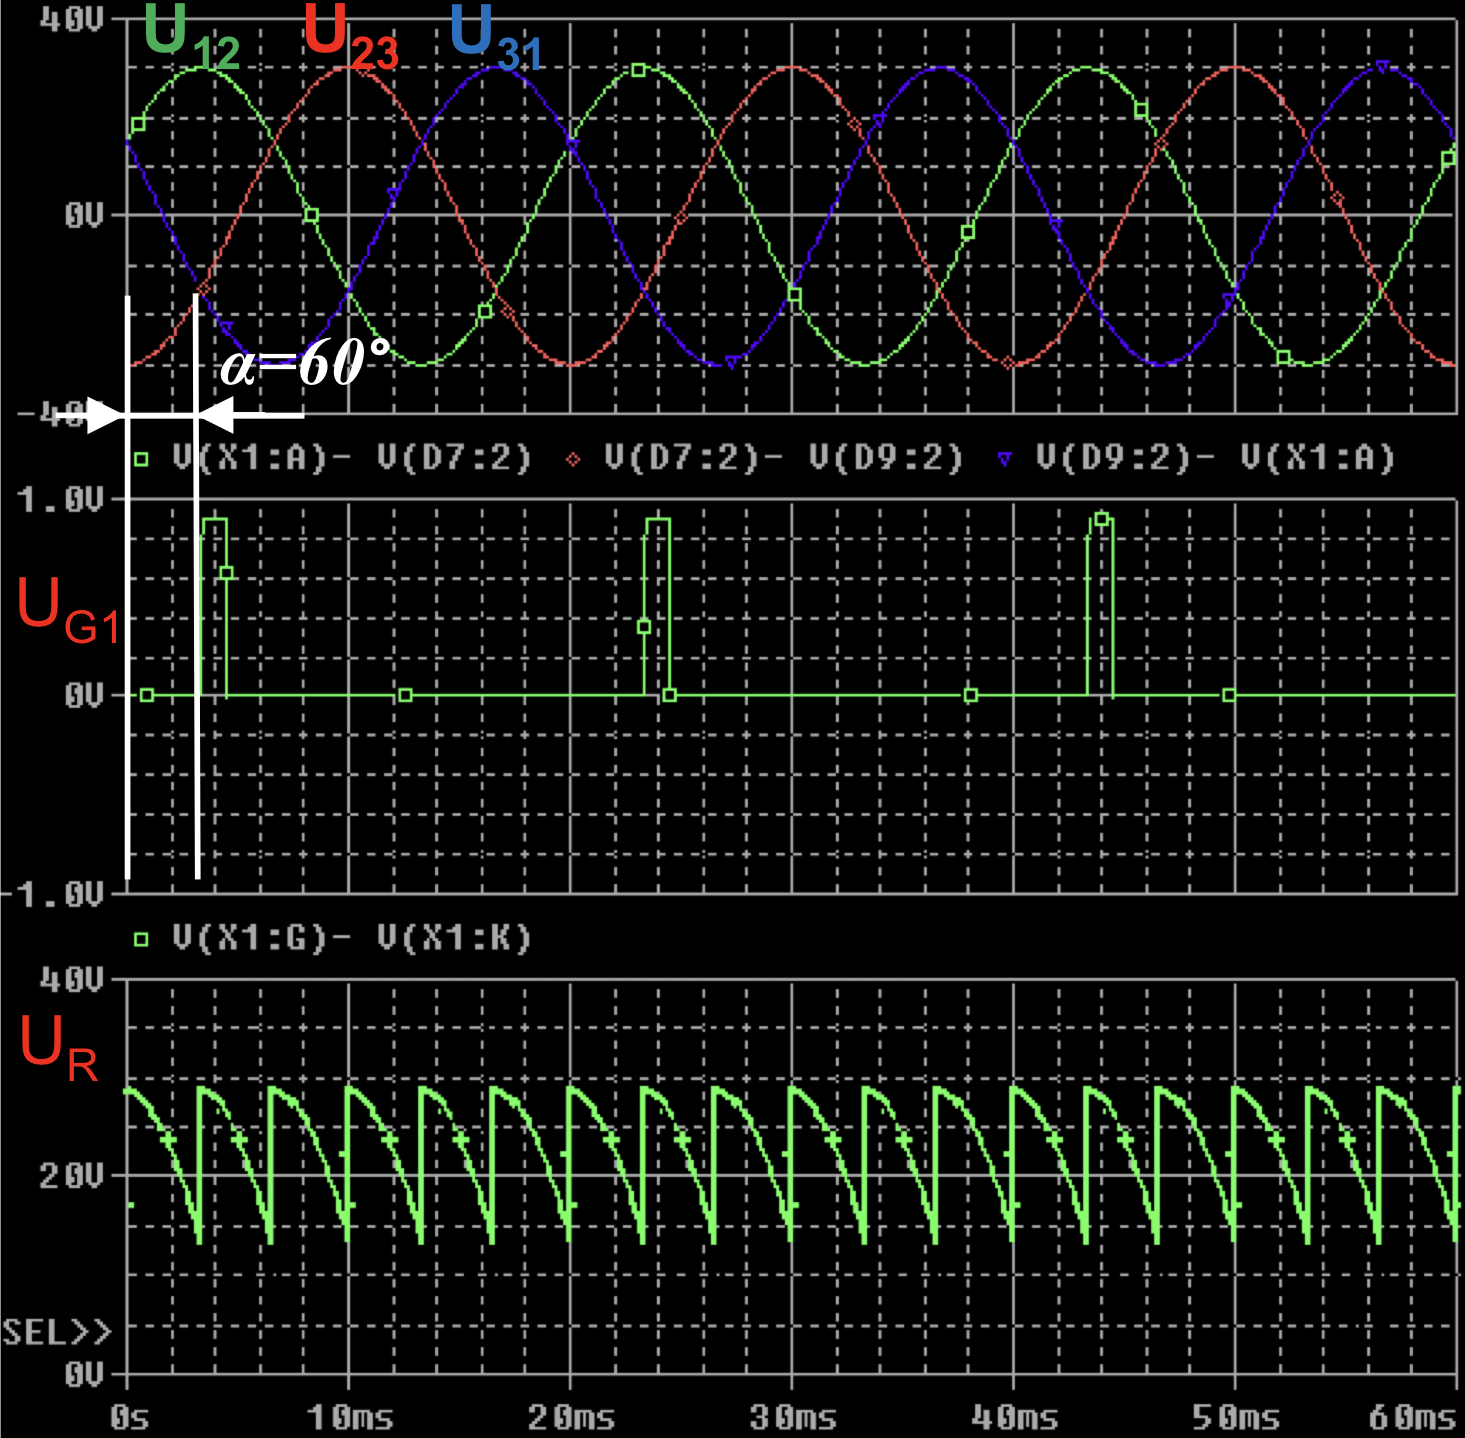
\includegraphics[width=0.85\linewidth]{images/B6C_Verlauf.png}
\end{center}
